\chapter{発話内容を考慮した偽音声検出}\label{ch:spc_cnt}
\section{目的}\label{sec:cnt_pur}
\subsection{形式の位置づけ}
音声を入力とする話者認識(Speaker Recognition)には、話者識別(Speaker Identification)と話者照合(Speaker Verification)という2種類の形式がある \cite{FURUI1997859,628714,5745552}。

話者識別は事前に登録した複数の候補者の中から提示された音声の話者を探索する1対nの推定問題であるのに対し、
話者照合では,提示された二つの音声が同一話者によるものか否かを推定する1対1の照合問題として定義する \cite{俵直弘2022}。
識別では、未知の話者を既知の話者のデータベースと比較し、最もよく一致する話者を識別結果として与える。
一方で照合では、音声サンプルが主張された人物によって話されたかどうかを判断するタスクと言える \cite{1561284}。
よって、本研究で行うなりすまし偽音声の検出は、話者照合に該当する。

また,話者認識は,登録時と照合時で同じ内容の音声を用いるテキスト依存型(text-dependent)と,
登録時と照合時で異なる内容の音声を用いるテキスト独立型(text-independent)に分類される \cite{俵直弘2022}。
ASVspoofにおけるなりすまし検出では、テキスト依存型の形式を取っている。
読み上げる音声は本人・偽いずれも新聞記事から引用した同一の文章を読み上げているため、
実際にSNS上で偽音声による偽情報が投稿された状況から乖離がある。
よって本研究では、テキスト独立型の話者照合を行う。

\subsection{検出対象の位置付け}
本研究の目的は、偽情報を話すなりすまし音声(偽音声)を自動で検出することである。
偽情報を話す偽音声には内容の確からしさと音声そのものの本人性という2種類の概念をもつ。
話す内容の確からしさは、事実か・偽情報かの2種がある。本来では事実ではないものの意図的なものではない誤情報もあるが、本章では考慮しない。
本人性は本人が話すか・本人以外がなりすましているかの2種がある。
本人以外がなりすます場合では機械による合成処理を含まない場合(声真似等)もあるが、
意図的に社会に不安を与える行為として行われにくいと考えられるため本章では考慮しない。

よって、偽情報を話すなりすまし音声を検出する場合、モデルへ入力する対象は内容の確からしさと本人性から以下の4種類が挙げられる。

\begin{itemize}
    \item 偽情報を話すなりすまし音声(検出したい対象)
    \item 事実を話すなりすまし音声
    \item 偽情報を話す本人音声
    \item 事実を話す本人音声
\end{itemize}

事実を話す本人音声は、検出したい対象である偽情報を話すなりすまし音声とは内容の確からしさ及び本人性の両方において、対極に位置する概念である。
本研究では、実験にて検出すべきでない対象として扱う。

事実を話すなりすまし音声は、主にマスメディアによるニュース記事の読み上げ(AIアナウンサー)が例として挙げられる\cite{nhk2020,nhkAnnual2020}。
マスメディアによる運用が行われているため、SNS上に投稿された場合は性質上一定の信憑性が見込まれて検出の必要性が薄いと判断し、本研究では扱わないこととした。

偽情報を話す本人音声は実際の例として演説や講演会、そして特殊詐欺などが挙げられる。
この場合は実際に話さなければならない都合上、SNS上での事例が偽情報を話すなりすまし音声に比べて変化が少ないほか、
先行研究として特殊詐欺の自動検出を目指した事例 \cite{近野恵2023}があるため、
検出したい対象に対して重要度が比較的高くないと判断し、本研究では扱わないこととした。

以上から、本研究の目的は事実を話す本人音声と偽情報を話すなりすまし音声の2種類の音声から検出を行う。

\section{手法}\label{sec:cnt_mtd}
\subsection{データセット作成手法}\label{ssc:spc_ds}
発話内容を考慮したモデルに分類させるため、
事実に基づく情報を読み上げる音声と事実と異なる偽情報を読み上げる音声を用意することにした。
読み上げる対象はMuMiNデータセットが保有する英語の偽情報ツイートとした \cite{10.1145/3477495.3531744}。
選定理由はデータセットからツイート文章とともに内容を埋め込みに変換した情報も得られることから、後述の提案手法への接続が容易に実現できるためである。

読み上げ手法はVITSを採用した \cite{pmlr-v139-kim21f}。
\cref{ch:rel_res}で紹介した文章から音声を生成するText-To-Speechの形式であることと、
生成性能が良好である点が示されている点、
そして音声生成学習においてLJSpeechデータセット \cite{ljspeech17}による事前学習済みモデルが公開されており、生成への活用が容易である点から採用した。

なお実験で使用するにあたって、SNS上での投稿を想定して音声が3分以内に収まるように
英単語数の上限を480に設定し、超過分は切除した上でVITSによる音声生成を行った。
ただしTwitterツイートは仕様上480文字までの制限があるため、今回実験で使用した音声長は最長でも24秒である。
データセットの統計は\cref{tb:dataset}の通りである。

\begin{table}[h]
    \centering
    \caption{実験で使用した偽音声データセットの統計}
    \begin{tabular}{lc}\hline
        項目 & 値\\\hline\hline
        ツイート件数 & 722\\
        最大単語数 & 50\\
        平均単語数 & 24.9\\
        平均音声長 [\si{s}] & 8.2\\\hline
    \end{tabular}
    \label{tb:dataset}
\end{table}

\subsection{検出手法}
発話内容を考慮したモデルを構築するために、文章埋め込みを入力にもつモデルを音声波形を扱う既存手法に追加する手法を提案する。提案手法全体の概観は\cref{fig:allmodel}の通りである。
音声波形を直接扱う既存手法として、
ASVspoofにてベースラインとして提供された \cite{WANG2020101114}RawNet2を採用した。
RawNet2はもともとRawNet \cite{jung19b_interspeech}から拡張された手法で、
いずれも発話レベルの特徴抽出と特徴拡張を単一モデルで完結させた上で分類を行う。
今回採用したRawNet2の構造は\cref{tb:rawnet2}の通りである。

\begin{figure}[ht]
    \centering
    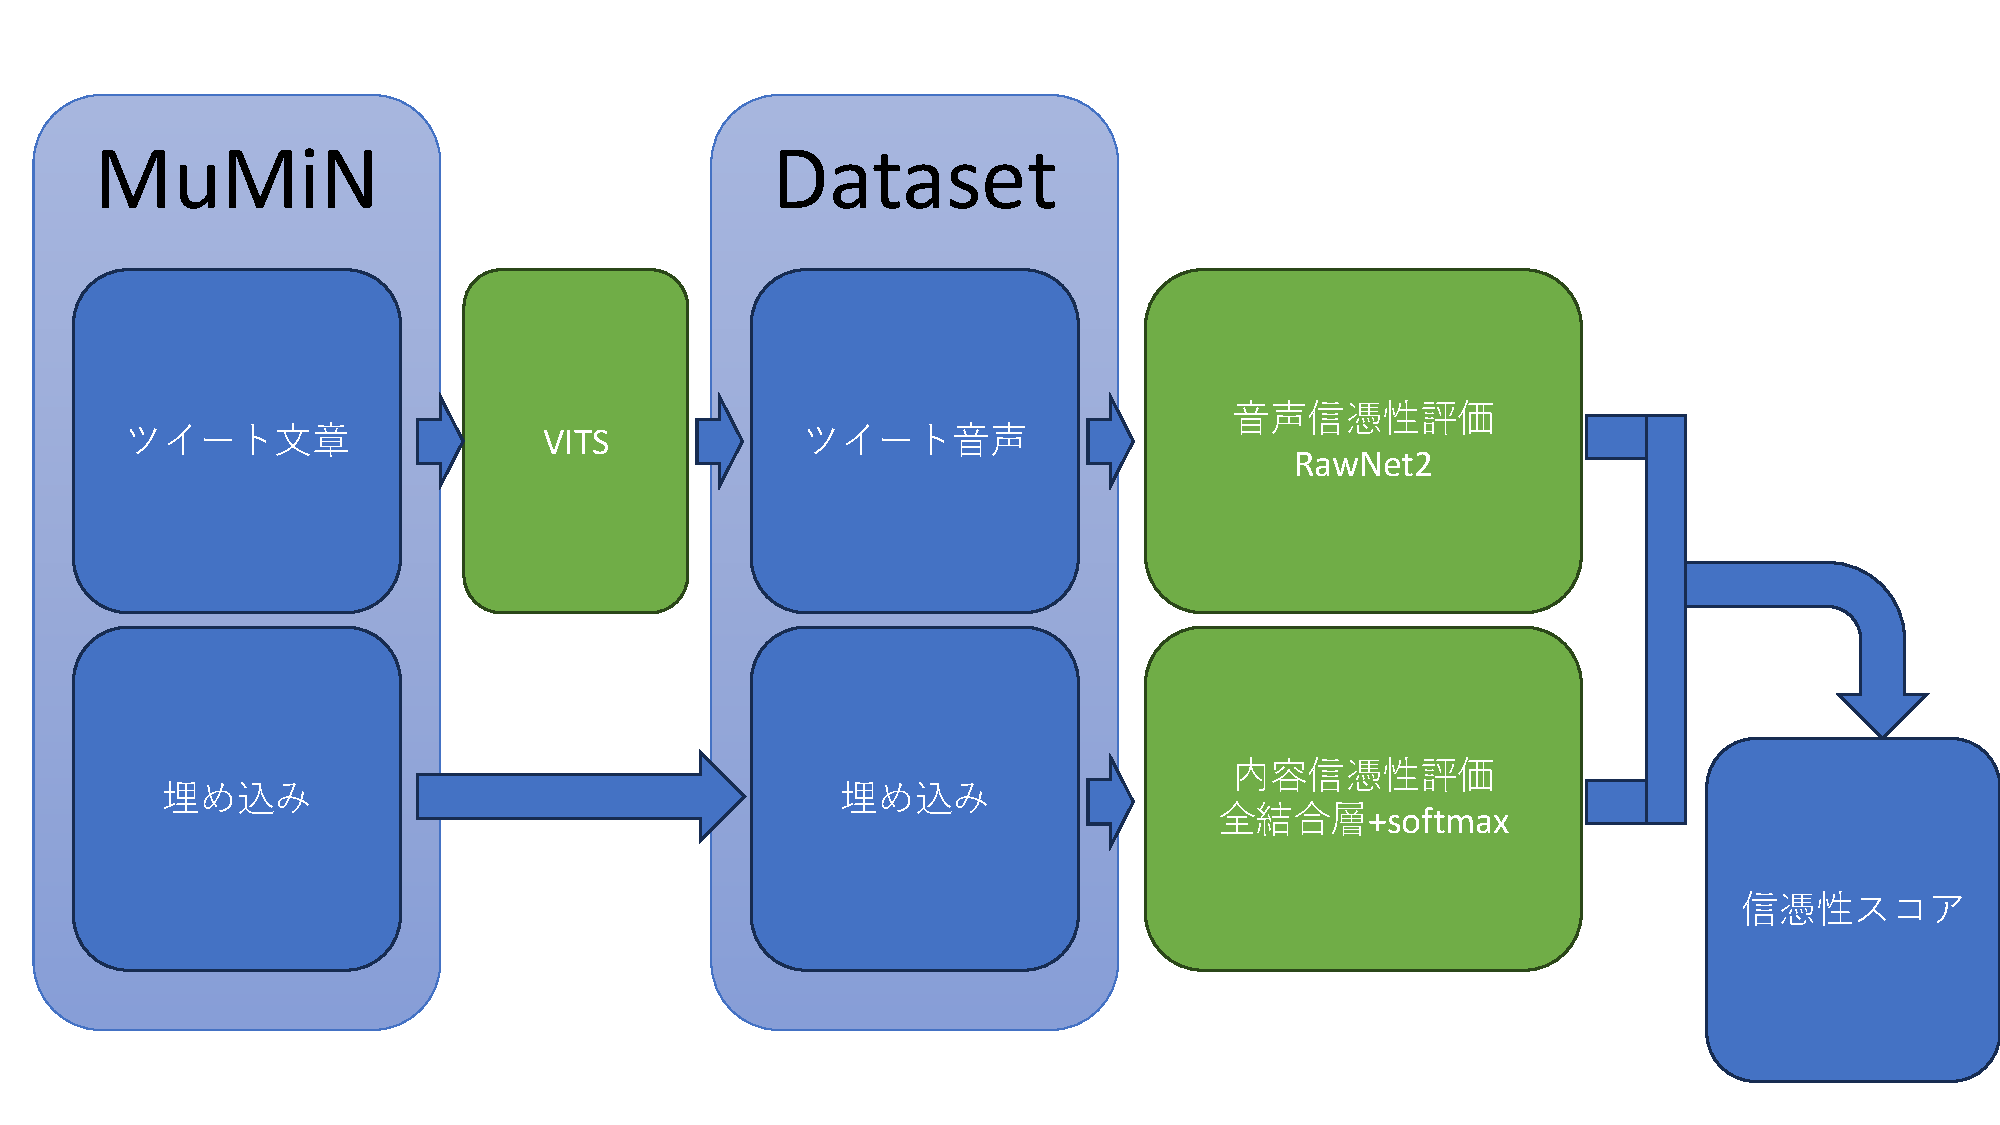
\includegraphics[width=\textwidth]{./figures/ieice_allFig.pdf}
    \caption{使用データセットの取得および提案手法の概観図。}
    \label{fig:allmodel}
\end{figure}


\begin{figure}[ht]
    \centering
    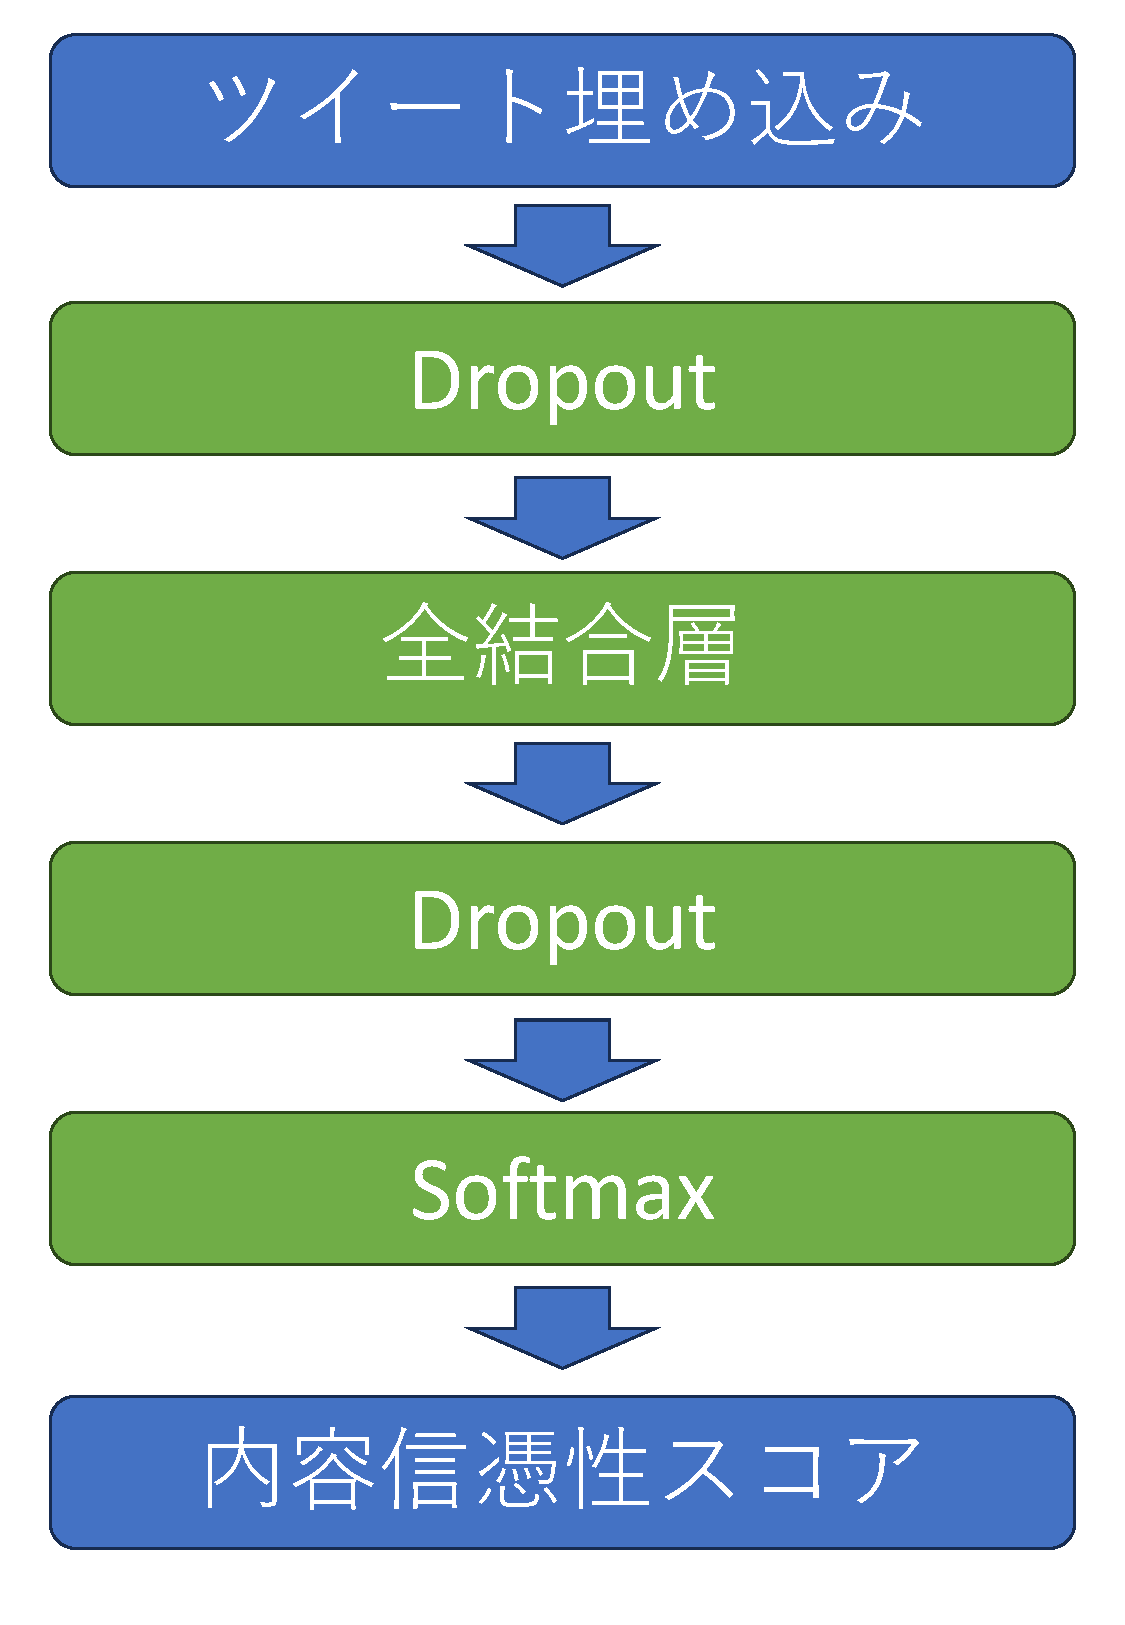
\includegraphics[width=0.5\textwidth]{./figures/ieice_nnfig.pdf} %TODO 次元情報追加
    \caption{提案手法における内容信憑性評価部分。}
    \label{fig:content}
\end{figure}

\begin{table}[ht]
    \centering
    \caption{ASVspoof 2019以降で採用されている \cite{9414234,yamagishi21_asvspoof}RawNet2の構造}
    \begin{tabular}{l@{}c@{}l}\hline
        層 & 入力 & 出力形式 \\\hline\hline
        \multirow{3}{*}{調整済Sincフィルタ} & 畳み込み(129,1,128) & \multirow{3}{*}{(21290, 128)}\\
        & 最大値プーリング(3) &\\
        & バッチ正規化(BN) \& LeakyReLU &\\\hline
        \multirow{6}{*}{残差ブロック}&\multirow{6}{*}{$\left\{\begin{array}{c}\rm{BN \& LeakyReLU}\\
        \rm{畳み込み(3,1,128)}\\
        \rm{BN \& LeakyReLU}\\
        \rm{畳み込み(3,1,128)}\\
        \rm{最大値プーリング(3)}\\
        \rm{特徴マップスケーリング(FMS)}\\\end{array}\right\}$}& \multirow{6}{*}{(2365, 128)}\\ \\ \\ \\ \\ \\\hline
        \multirow{6}{*}{残差ブロック}&\multirow{6}{*}{$\left\{\begin{array}{c}\rm{BN \& LeakyReLU}\\
        \rm{畳み込み(3,1,128)}\\
        \rm{BN \& LeakyReLU}\\
        \rm{畳み込み(3,1,128)}\\
        \rm{最大値プーリング(3)}\\
        \rm{FMS}\\\end{array}\right\}$}& \multirow{6}{*}{(29, 512)}\\ \\ \\ \\ \\ \\\hline
        ゲート付き回帰型ユニット&GRU(1024)&(1024)\\\hline
        全結合層&1024&(1024)\\\hline
        Output&1024&2\\\hline
        %& Maxpooling(3) &\\
    \end{tabular}
    \label{tb:rawnet2}
\end{table}


提案手法は、MuMiNデータセット内にてツイートに書かれた言語に対応したBERTベースの変換モデル \cite{lewis-etal-2020-bart}を適用したツイート埋め込みを入力に、ニューラルネットワークを介して内容の信憑性を評価する。
具体的な内容信憑性評価部分の流れは\cref{fig:content}の通りである。
最終的な信憑性スコアは音声信憑性評価による出力と内容信憑性評価による出力の平均値とした。
追加部分が音声を入力に使わなかった理由として、TTSによって得た合成音声は自動音声認識(Automatic Speech Recognition; ASR)による書き起こしが容易に得られることが想定でき、省略可能と考えたためである。
%今後VCによる変換も対象に入れる場合も想定し、音声を入力としてASRから発話内容を得る形への拡張も想定している。

\section{予備実験: 新型音声合成手法に対する既存検出手法の検証}
\subsection{実験内容}
\subsection{結果}
\section{本実験: 発話内容考慮による検出性能改善の検証}\label{sec:cnt_main}
\subsection{実験内容}
発話内容も含めて音声の信憑性を評価する手法の有効性を検証するために、
同じ合成音声でありながら事実に基づく情報とそうでない情報を真偽分類する実験を行った。
具体的なデータセット取得の手続き\cref{ssc:spc_ds}を参照のこと。
なおデータセット内の各ツイートのラベルはfactual/fakeの2種類である。
RawNet2は事前学習としてASVspoof 2021にて提供されたオンライン環境を想定した音声セットであるDFデータセットで学習済のものを使用した。
これはオンライン上に投稿された状況を想定した2019年までに提案された手法による合成音声から構成される。
また内容信憑性評価部分も含めた学習からテストまでの流れは学習/検証/テストの比率0.7:0.1:0.2の割合で分割して行った。学習エポック数は10だった。

評価指標は等価エラー率(Equal Error Rate; EER)を採用した。
これは真偽判断の閾値を本人拒否率(False Rejection Rate; FRR)と他人受入率(False Acceptance Rate; FAR)が同値になるように調整したときのエラー率を示したものである。
この2値は以下の式によって導出される。
\begin{eqnarray}
    FRR = \frac{FN}{FN+TP} \\
    FAR = \frac{FP}{FP+TN}
\end{eqnarray}

今回の実験でTP(True Positive)は偽情報を話す合成音声を正しく虚偽と検出できた回数を示し、
FN(False Negative)は偽情報を話す合成音声を誤って事実と分類した回数を示し、
FP(False Positive)は事実を話す合成音声に誤って虚偽と検出した回数を示す。

実験では提案手法の有効性を確認するために、
音声のみで分類を行った場合の結果と比較した。

\subsection{結果}\label{sec:cnt_res}
実験によって音声を分類した結果は\cref{tb:result}の通りである。
音声のみを入力として扱った場合、等価エラー率(EER)は50.7\%だった。
EERが50\%であることは、コイントスによって決定することとと同義であることから、
%2019年までの音声合成手法によって訓練されたRawNet2では、
%VITSによる音声を識別することが限りなく難しいことを示している。
%自明であるが、
内容の真偽に関係なく、発話音声か合成音声かを区別するように訓練されたRawNet2では、
内容が真の合成音声と内容が偽の合成音声とを区別することはできなかった。
一方で、内容評価を行う部分を付加した場合、
EERは44.59\%まで改善がみられた。

\begin{table}[h]
    \caption{事実に基づく情報と事実と異なる偽情報を話す合成音声を真偽分類した結果。}
    \centering
    \begin{tabular}{l|c}\hline
       モデル形態 & 等価エラー率(EER)[\%] \\\hline\hline
       音声評価 (RawNet2)のみ & 50.7\\
       提案手法(内容評価を伴う場合) & \textbf{44.6}\\\hline
    \end{tabular}
    \label{tb:result}
\end{table}

\section{考察}\label{sec:cnt_evl}

